\chapter{Tests und Experimente}
\label{cha:tests}

Im Kapitel Tests und Experimente werden unterschiedliche Hyperparameter-Konfigurationen auf ihre Auswirkungen getestet. Außerdem wird mit unterschiedlichen
Netzwerk-Architekturen die Performanz auf Geräten mit leistungsarmer Hardware gemessen.

\section{Auswirkungen der Hyperparameter}

Im Folgenden werden unterschiedliche Kombinationen der Gewichtungsparameter Content-Weight $ \alpha $, Style-Weight $ \beta $ und Total-Variation-Weight $ \gamma $ getestet. Dabei wird als Inhaltsbild  eine eigene Abbildung der HTW-Berlin benutzt. Als Stilbild wird das Kunstwerk \textit{The Starry Night} des Künstlers Vincent Van Gogh und \textit{The Scream} von Edvard Munch verwendet. Die generierten Bilder entsprechen einer Größe von 768 * 768 Pixeln. Die restlichen Hyperparameter werden aus dem Kapitel Methodologie \ref{sec:method_neural_style_transfer} übernommen.

\pagebreak

\subsection{Experiment 1: Starry Night}

In diesem Experiment wird das Stilbild The Starry Night von Vincent Van Gogh verwendet.

\begin{figure}[H]
    \centering
    \begin{subfigure}[h]{0.20\textwidth}
        \centering
        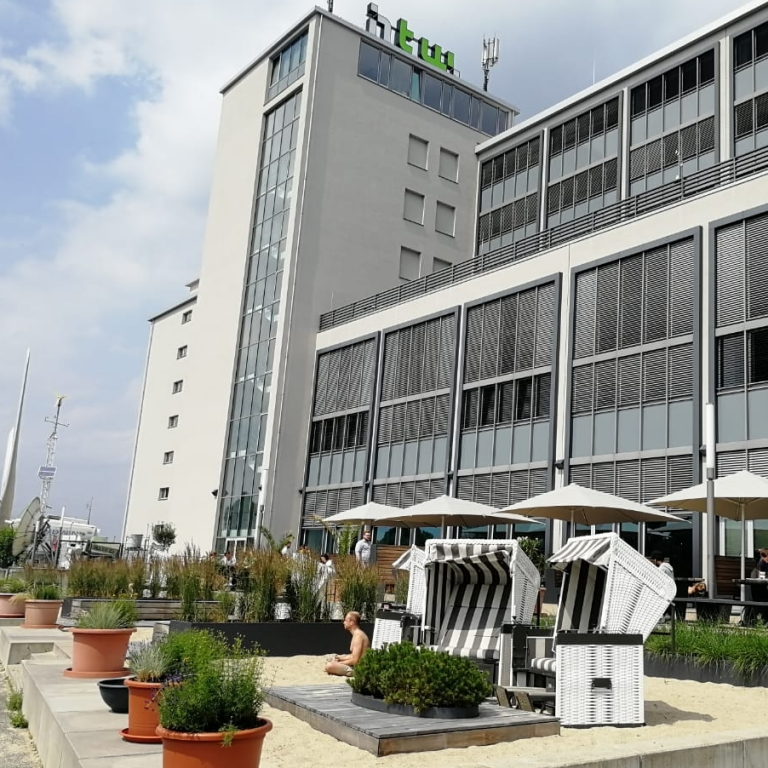
\includegraphics[width=\textwidth]{resources/content/content/htw-768x768.jpg}
    \end{subfigure}
    \begin{subfigure}[h]{0.20\textwidth}
        \centering
        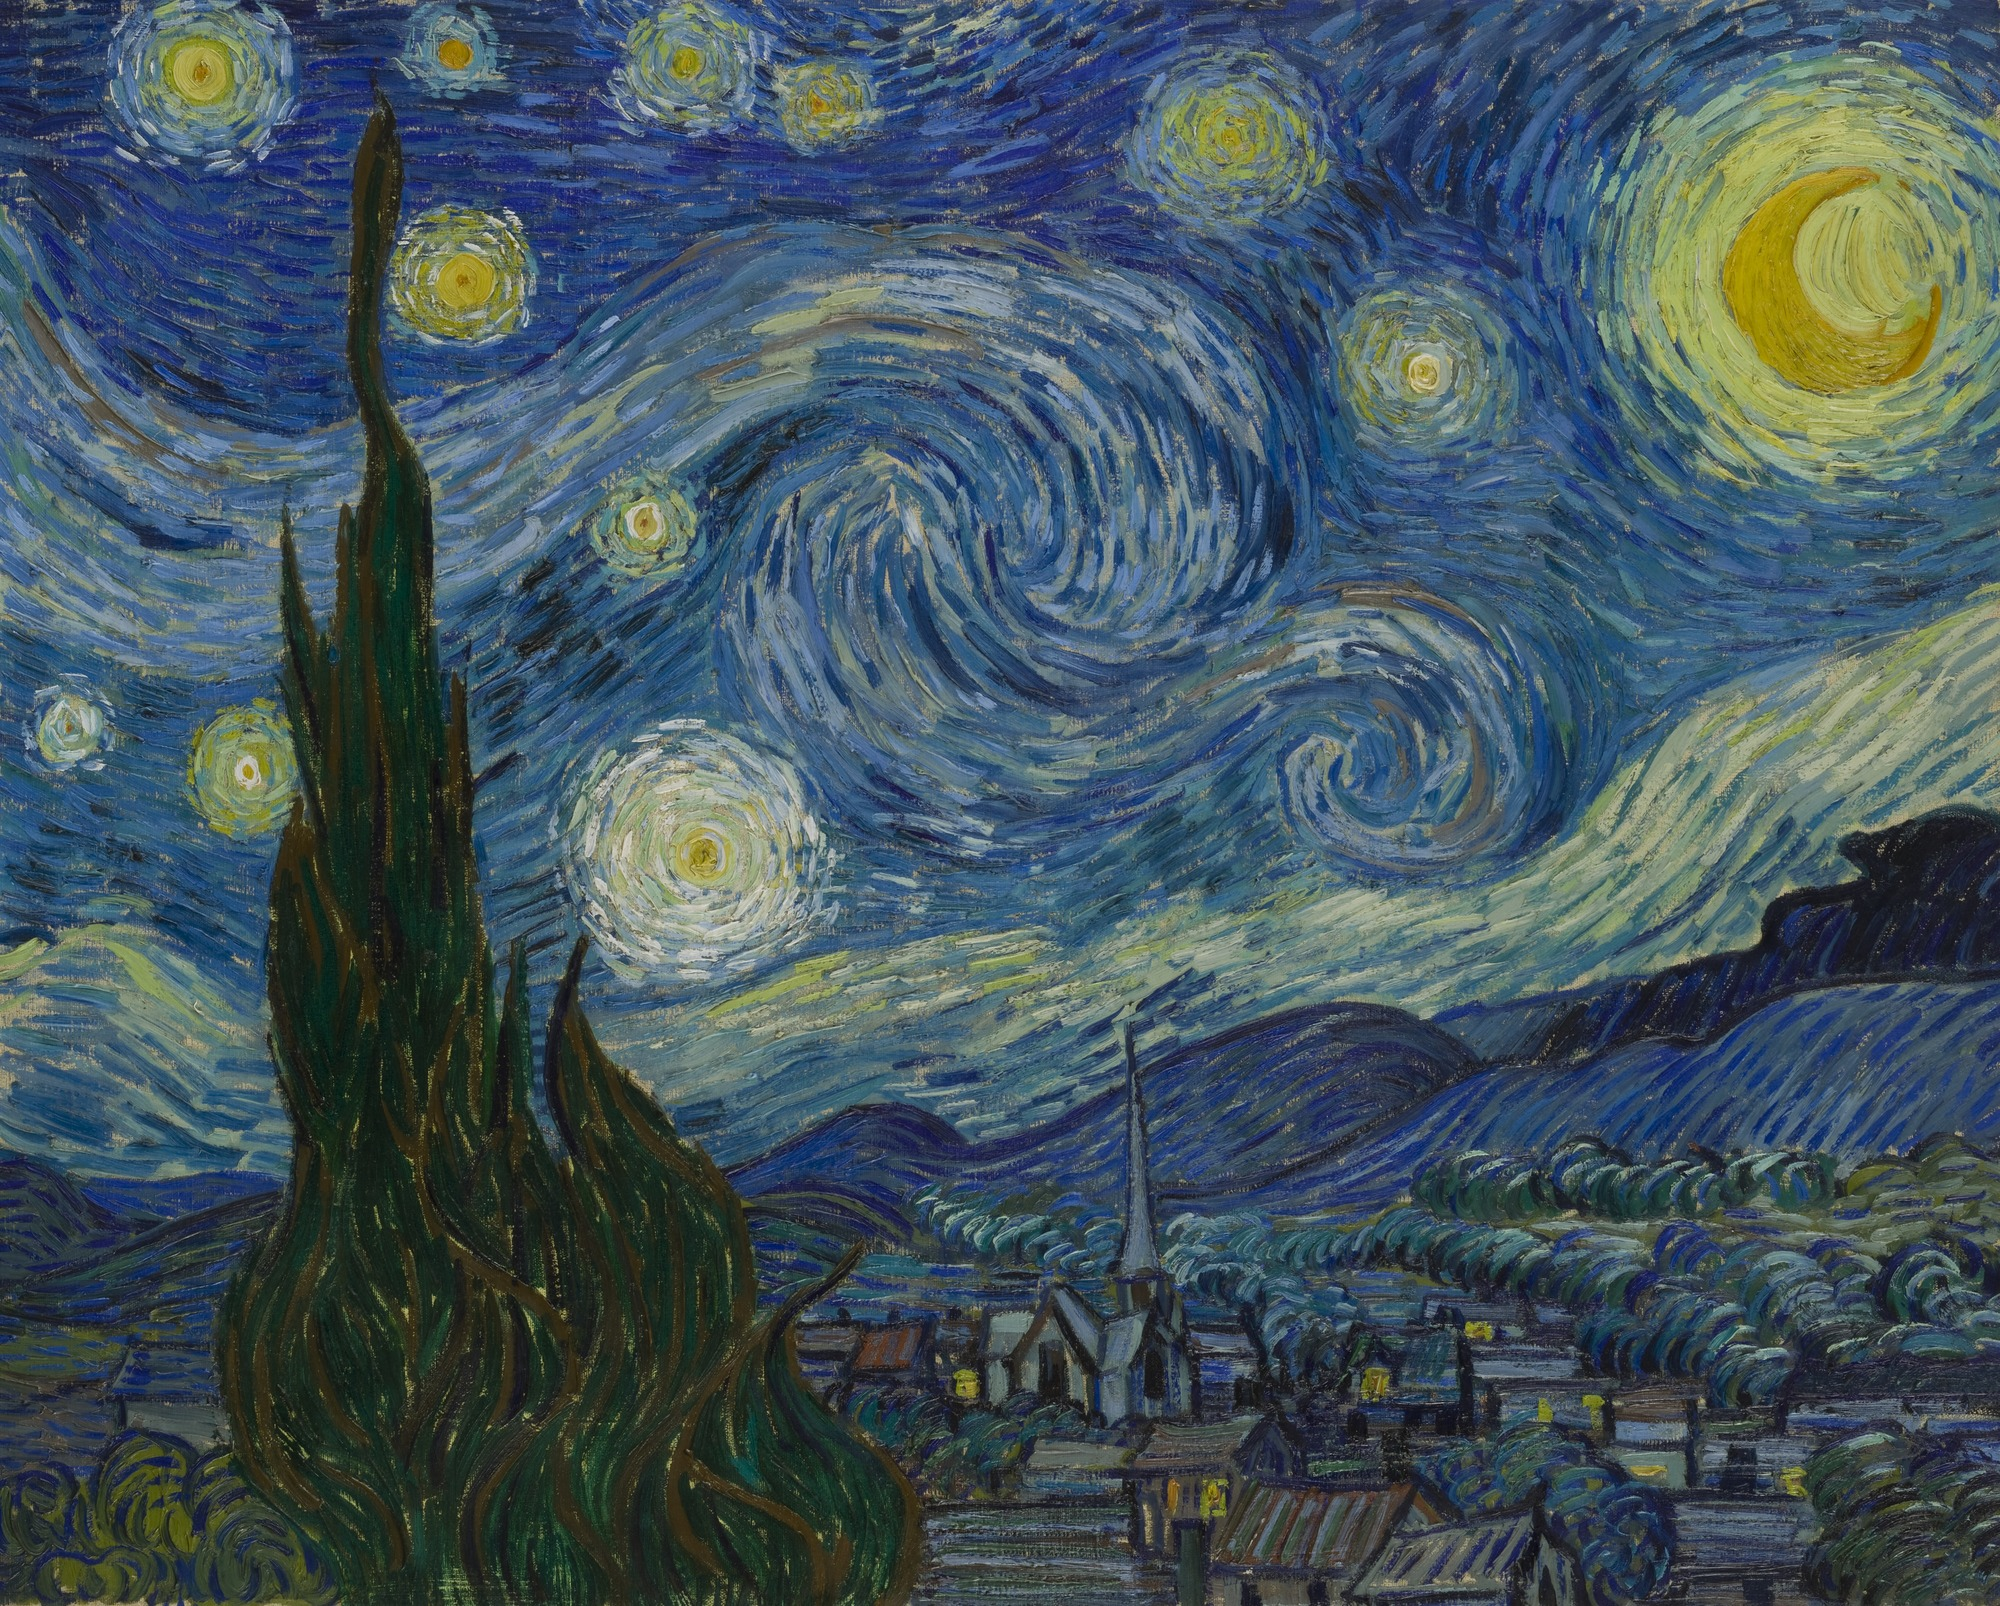
\includegraphics[width=\textwidth]{resources/content/style/starry_night.jpg}
    \end{subfigure}
    \caption{HTW kombiniert mit The Starry Night \cite{the_starry_night_img}}
\end{figure}

In der ersten Abbildungen werden die verschiedenen
Stilgewichtungen $ \beta = 10^{5} $, $ \beta = 10^{6} $, $ \beta = 10^{7} $, $ \beta = 10^{8} $ und $ \beta = 10^{9} $ für The Starry Night getestet.

\begin{figure}[H]
    \centering
    \begin{subfigure}[h]{0.15\textwidth}
        \centering
        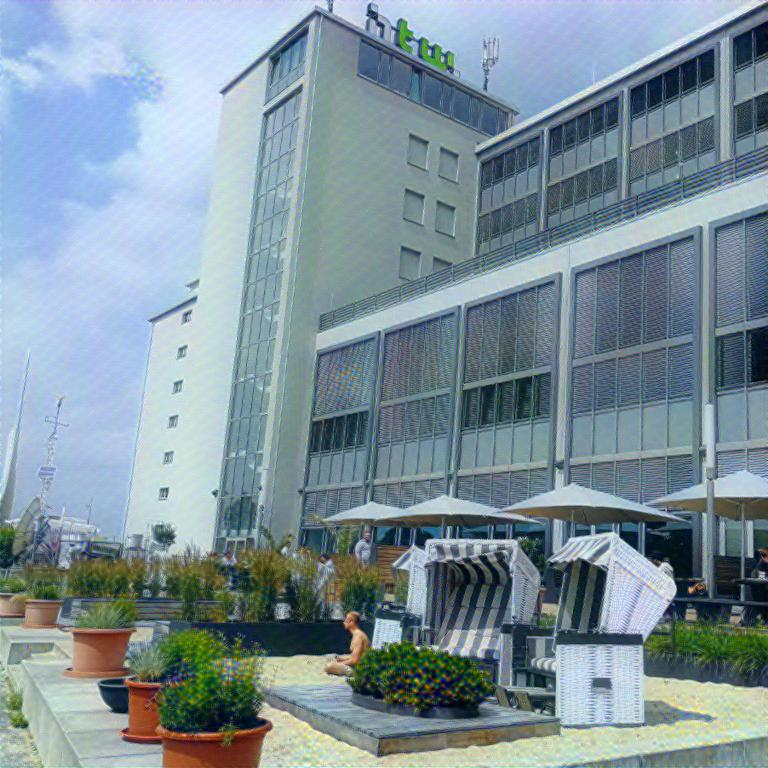
\includegraphics[width=\textwidth]{resources/content/experiments/a__starry_night__768x768__style-weight_1e+05__tv-weight_0e+00.jpg}
    \end{subfigure}
    \begin{subfigure}[h]{0.15\textwidth}
        \centering
        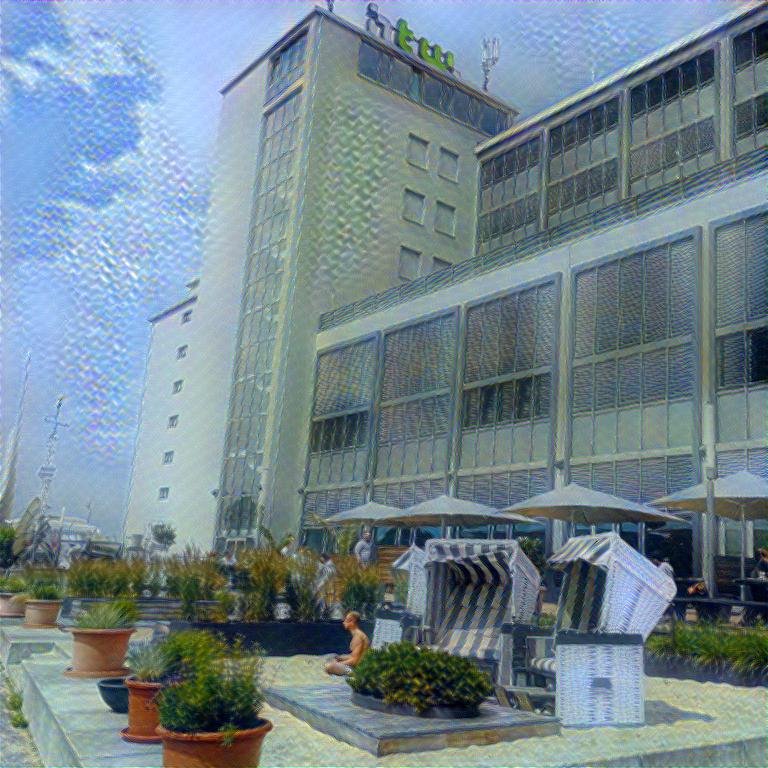
\includegraphics[width=\textwidth]{resources/content/experiments/a__starry_night__768x768__style-weight_1e+06__tv-weight_0e+00.jpg}
    \end{subfigure}
    \begin{subfigure}[h]{0.15\textwidth}
        \centering
        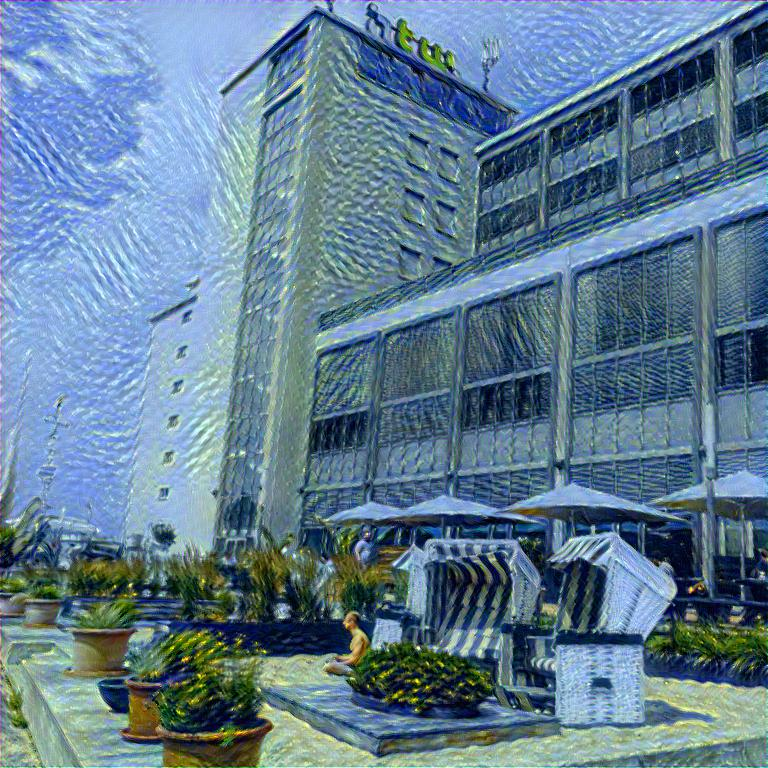
\includegraphics[width=\textwidth]{resources/content/experiments/a__starry_night__768x768__style-weight_1e+07__tv-weight_0e+00.jpg}
    \end{subfigure}
    \begin{subfigure}[h]{0.15\textwidth}
        \centering
        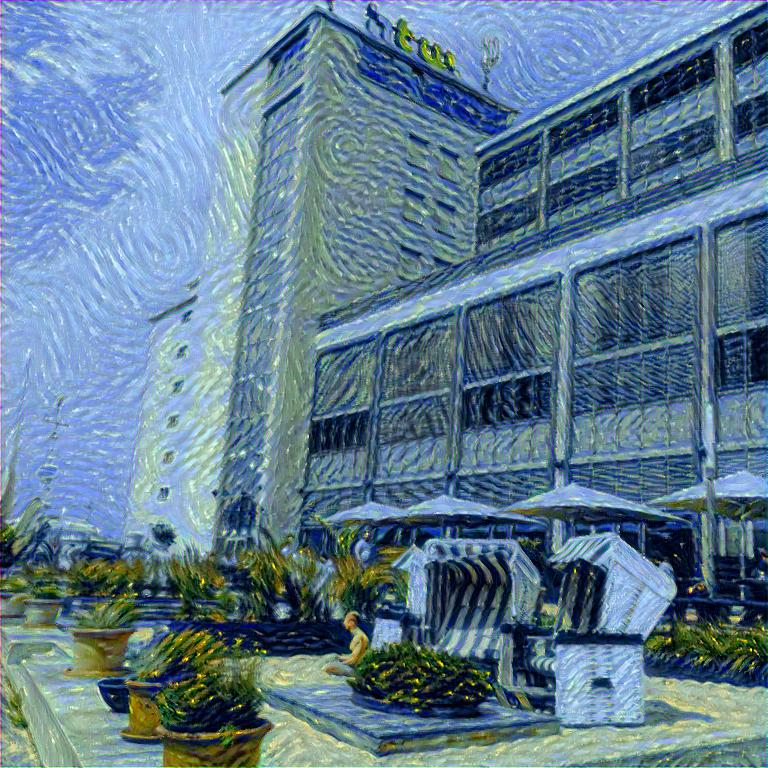
\includegraphics[width=\textwidth]{resources/content/experiments/a__starry_night__768x768__style-weight_1e+08__tv-weight_0e+00.jpg}
    \end{subfigure}
    \begin{subfigure}[h]{0.15\textwidth}
        \centering
        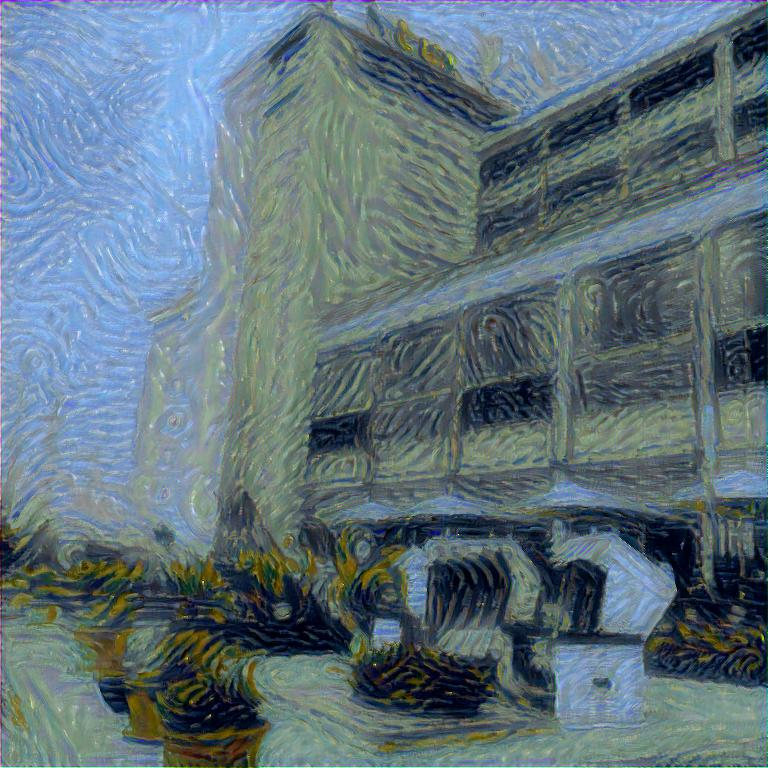
\includegraphics[width=\textwidth]{resources/content/experiments/a__starry_night__768x768__style-weight_1e+09__tv-weight_0e+00.jpg}
    \end{subfigure}
    \caption{The Starry Night mit $ \alpha = 1 $, $ \beta = 10^{5} - 10^{9} $, $ \gamma = 0 $}
\end{figure}

In der zweiten Abbildungen werden die verschiedenen Total-Variation-Gewichtungen $ \gamma = 10^{-7} $, $ \gamma = 10^{-6} $, $ \gamma = 10^{-5} $, $ \gamma = 10^{-4} $ und $ \gamma = 10^{-3} $  für Starry Night getestet.

\begin{figure}[H]
    \centering
    \begin{subfigure}[h]{0.15\textwidth}
        \centering
        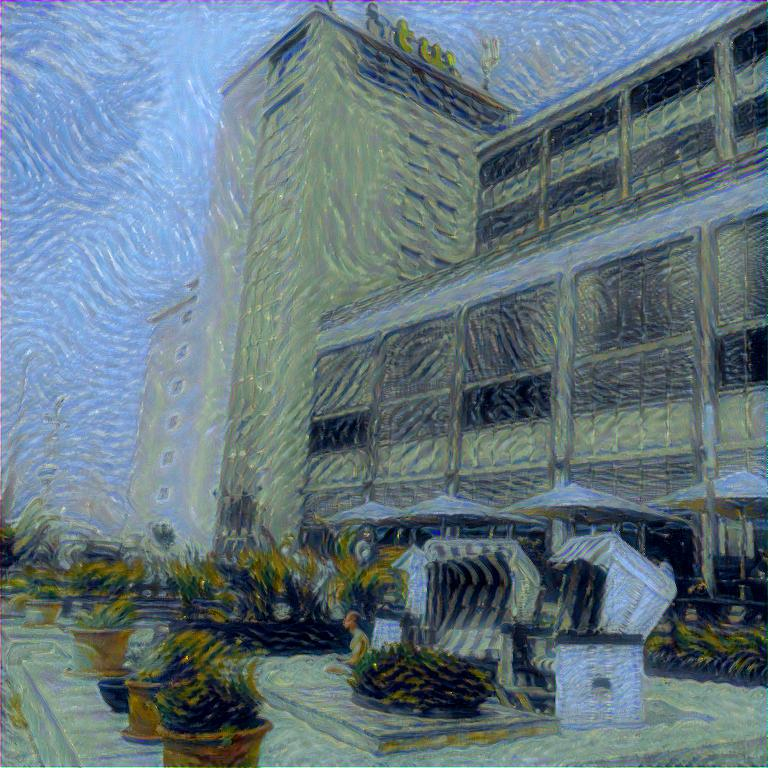
\includegraphics[width=\textwidth]{resources/content/experiments/b__starry_night__768x768__style-weight_1e+08__tv-weight_1e-07.jpg}
    \end{subfigure}
    \begin{subfigure}[h]{0.15\textwidth}
        \centering
        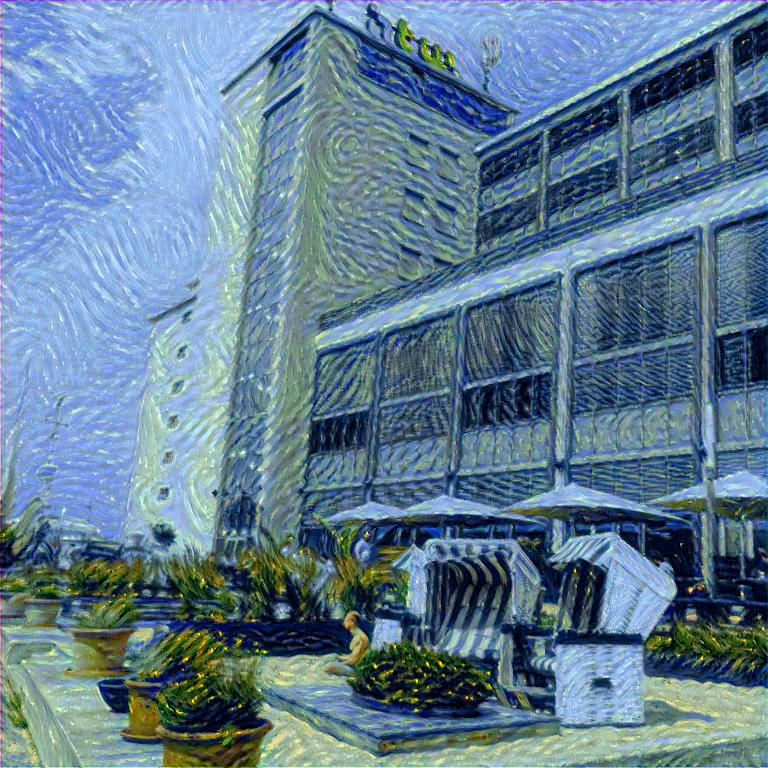
\includegraphics[width=\textwidth]{resources/content/experiments/b__starry_night__768x768__style-weight_1e+08__tv-weight_1e-06.jpg}
    \end{subfigure}
    \begin{subfigure}[h]{0.15\textwidth}
        \centering
        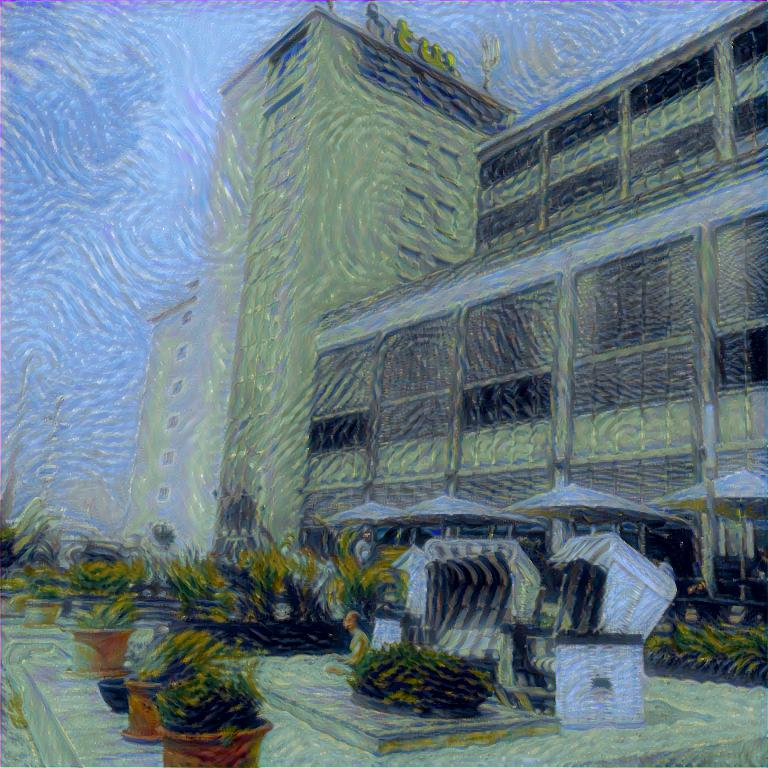
\includegraphics[width=\textwidth]{resources/content/experiments/b__starry_night__768x768__style-weight_1e+08__tv-weight_1e-05.jpg}
    \end{subfigure}
    \begin{subfigure}[h]{0.15\textwidth}
        \centering
        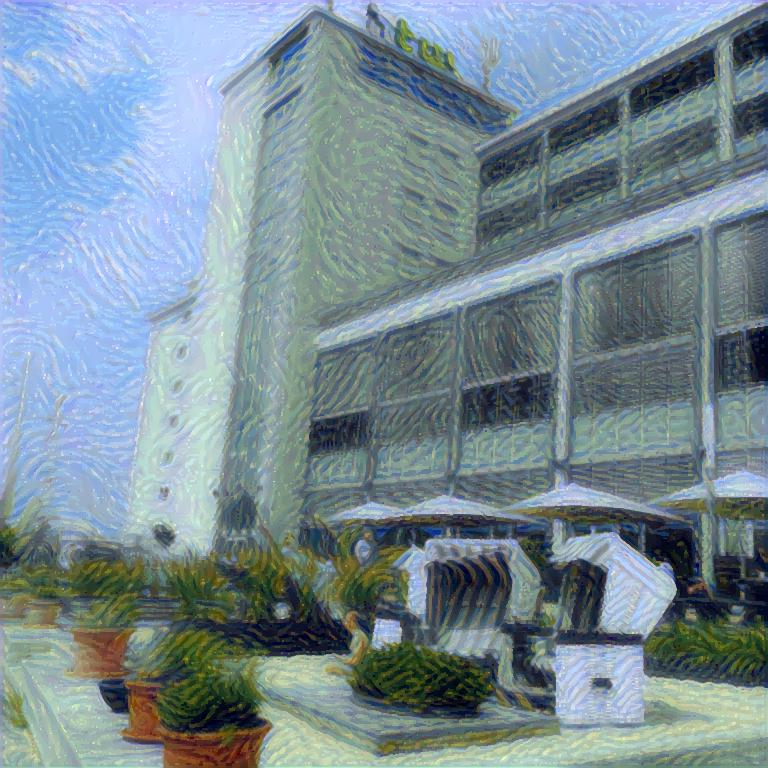
\includegraphics[width=\textwidth]{resources/content/experiments/b__starry_night__768x768__style-weight_1e+08__tv-weight_1e-04.jpg}
    \end{subfigure}
    \begin{subfigure}[h]{0.15\textwidth}
        \centering
        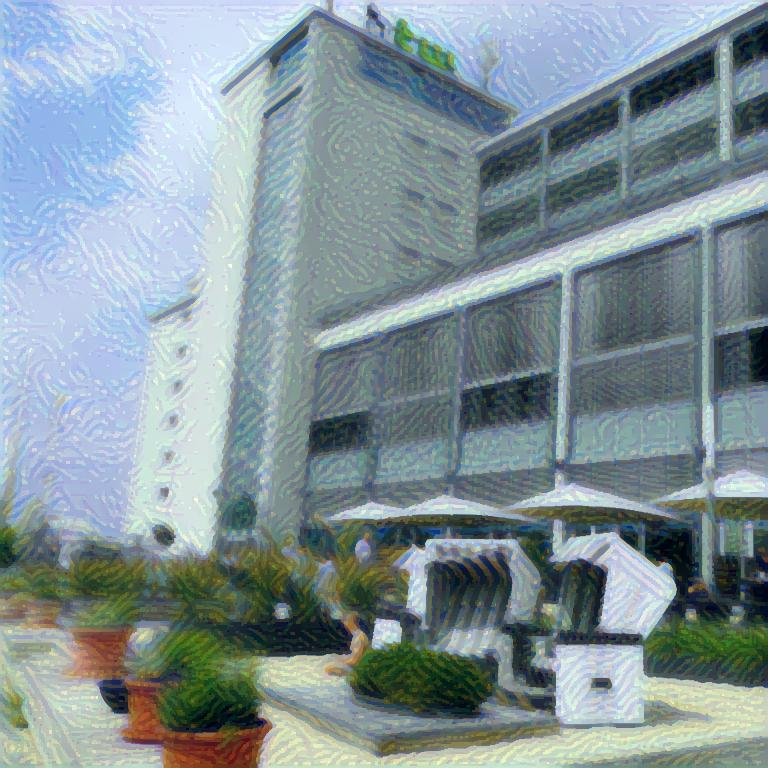
\includegraphics[width=\textwidth]{resources/content/experiments/b__starry_night__768x768__style-weight_1e+08__tv-weight_1e-03.jpg}
    \end{subfigure}
    \caption{Starry Night mit $ \alpha = 1 $, $ \beta = 10^{8} $, $ \gamma = 10^{-7} - 10^{-3} $}
\end{figure}

\pagebreak

\subsection{Experiment 2: The Scream}

\begin{figure}[H]
    \centering
    \begin{subfigure}[h]{0.20\textwidth}
        \centering
        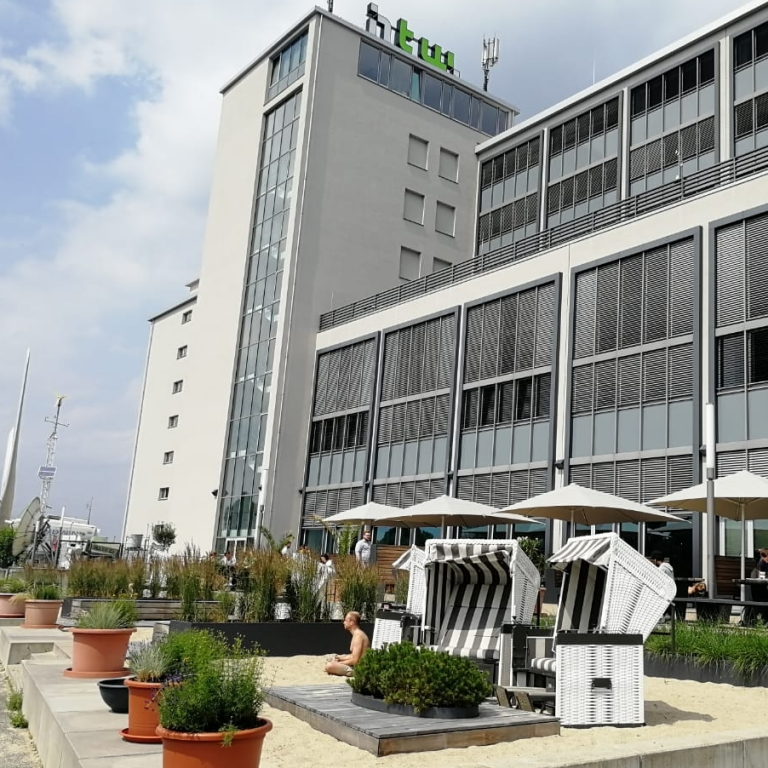
\includegraphics[width=\textwidth]{resources/content/content/htw-768x768.jpg}
    \end{subfigure}
    \begin{subfigure}[h]{0.20\textwidth}
        \centering
        \includegraphics[width=\textwidth]{resources/content/style/the_scream.jpg}
    \end{subfigure}
    \caption{HTW kombiniert mit The Scream \cite{the_scream_img}}
\end{figure}


In der ersten Abbildungen werden verschiedene die verschiedenen  \\
Stilgewichtungen $ \beta = 10^{5} $, $ \beta = 10^{6} $, $ \beta = 10^{7} $, $ \beta = 10^{8} $ und $ \beta = 10^{9} $ für The Scream getestet.

\begin{figure}[H]
    \centering
    \begin{subfigure}[h]{0.15\textwidth}
        \centering
        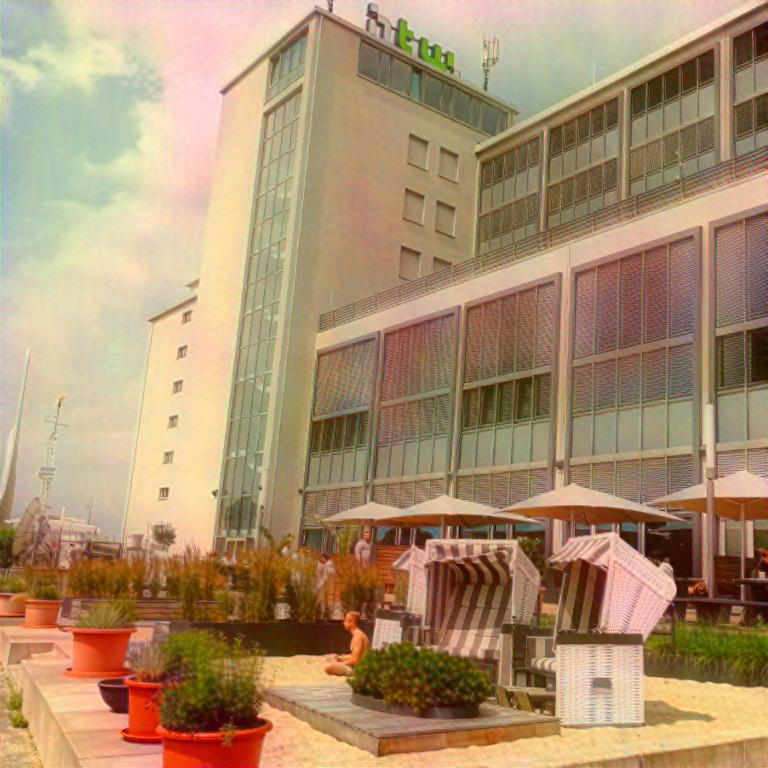
\includegraphics[width=\textwidth]{resources/content/experiments/a__the_scream__768x768__style-weight_1e+05__tv-weight_0e+00.jpg}
    \end{subfigure}
    \begin{subfigure}[h]{0.15\textwidth}
        \centering
        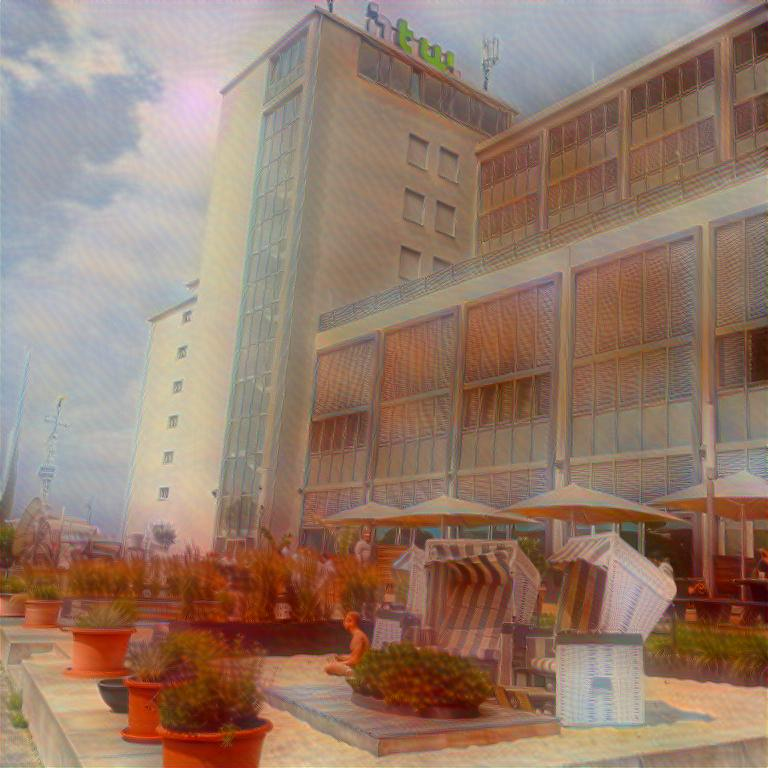
\includegraphics[width=\textwidth]{resources/content/experiments/a__the_scream__768x768__style-weight_1e+06__tv-weight_0e+00.jpg}
    \end{subfigure}
    \begin{subfigure}[h]{0.15\textwidth}
        \centering
        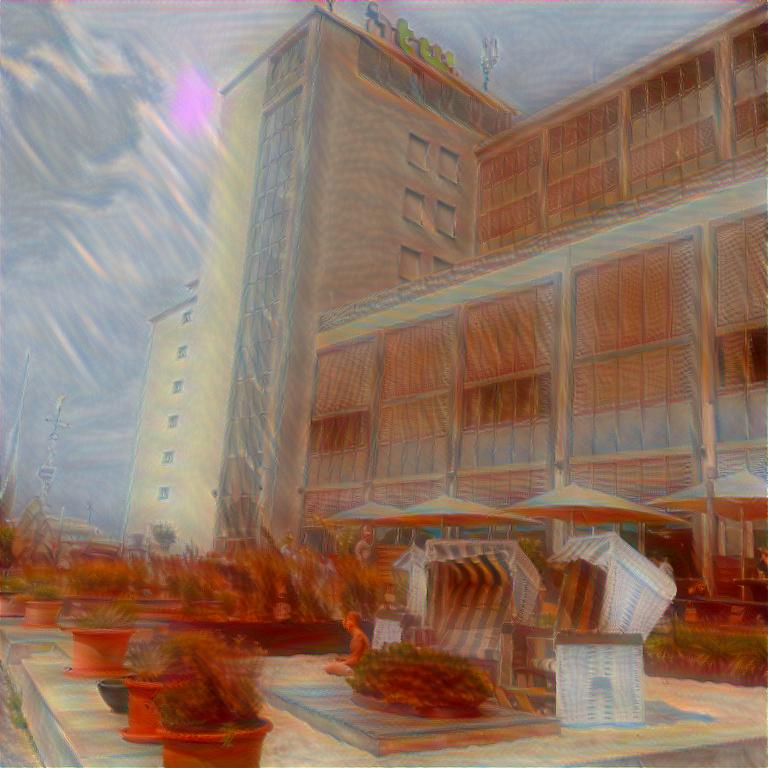
\includegraphics[width=\textwidth]{resources/content/experiments/a__the_scream__768x768__style-weight_1e+07__tv-weight_0e+00.jpg}
    \end{subfigure}
    \begin{subfigure}[h]{0.15\textwidth}
        \centering
        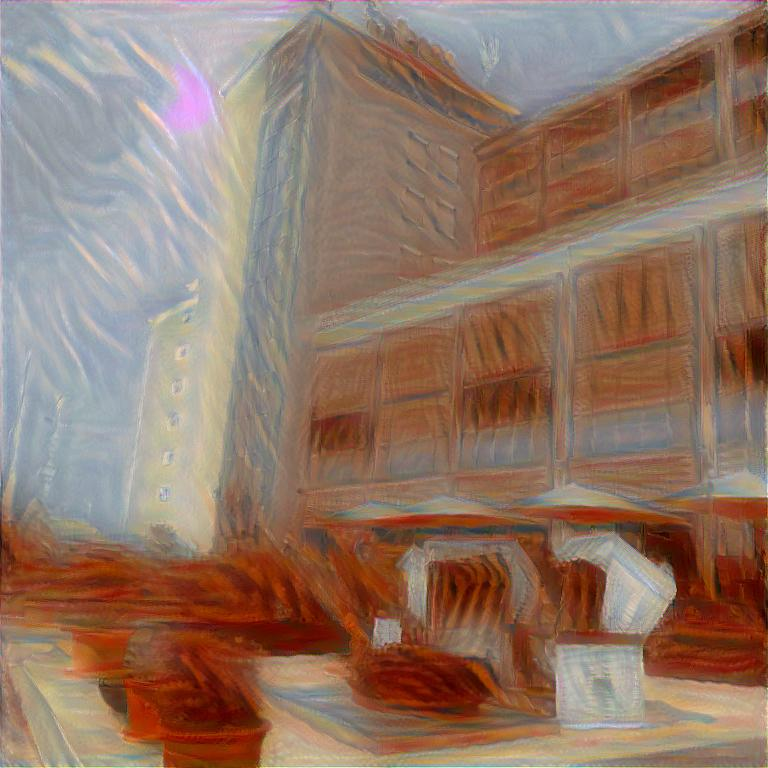
\includegraphics[width=\textwidth]{resources/content/experiments/a__the_scream__768x768__style-weight_1e+08__tv-weight_0e+00.jpg}
    \end{subfigure}
    \begin{subfigure}[h]{0.15\textwidth}
        \centering
        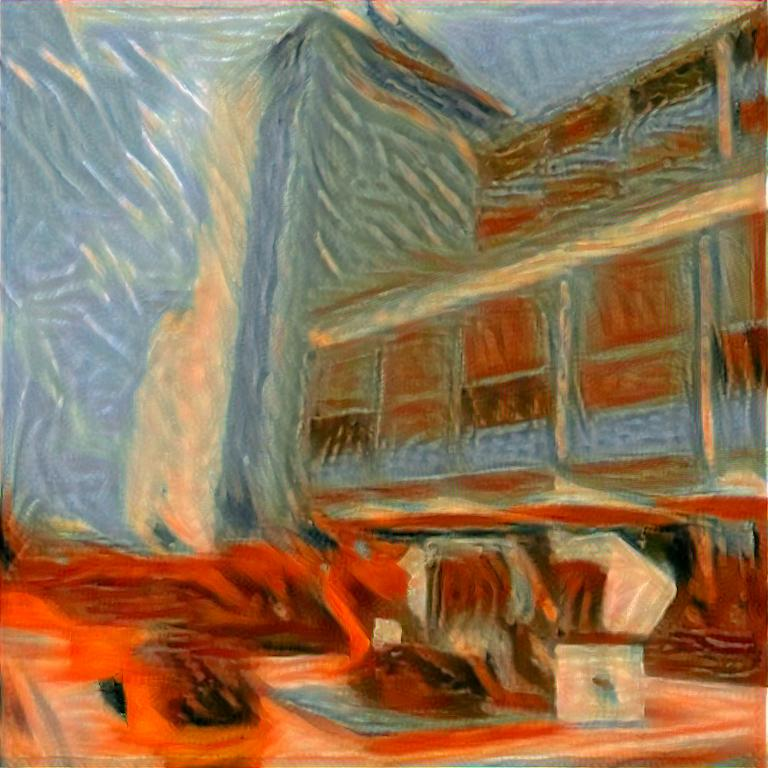
\includegraphics[width=\textwidth]{resources/content/experiments/a__the_scream__768x768__style-weight_1e+09__tv-weight_0e+00.jpg}
    \end{subfigure}
    \caption{The Scream mit $ \alpha = 1 $, $ \beta = 10^{5} - 10^{9} $, $ \gamma = 0 $}
\end{figure}

In der zweiten Abbildungen werden verschiedene die verschiedenen Total-Variation-Gewichtungen $ \gamma = 10^{-7} $, $ \gamma = 10^{-6} $, $ \gamma = 10^{-5} $, $ \gamma = 10^{-4} $ und $ \gamma = 10^{-3} $ für The Scream getestet.

\begin{figure}[H]
    \centering
    \begin{subfigure}[h]{0.15\textwidth}
        \centering
        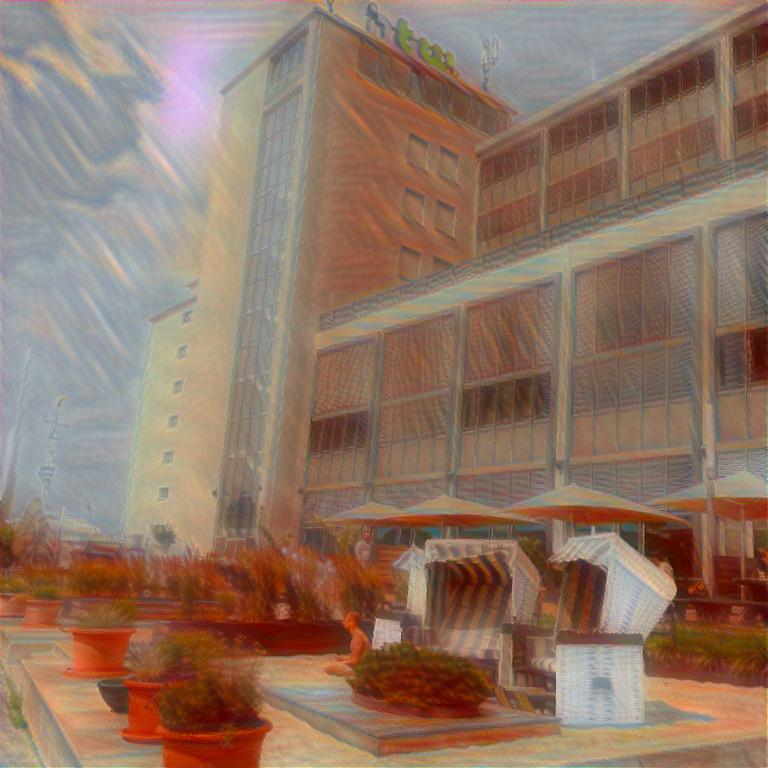
\includegraphics[width=\textwidth]{resources/content/experiments/b__the_scream__768x768__style-weight_1e+07__tv-weight_1e-07.jpg}
    \end{subfigure}
    \begin{subfigure}[h]{0.15\textwidth}
        \centering
        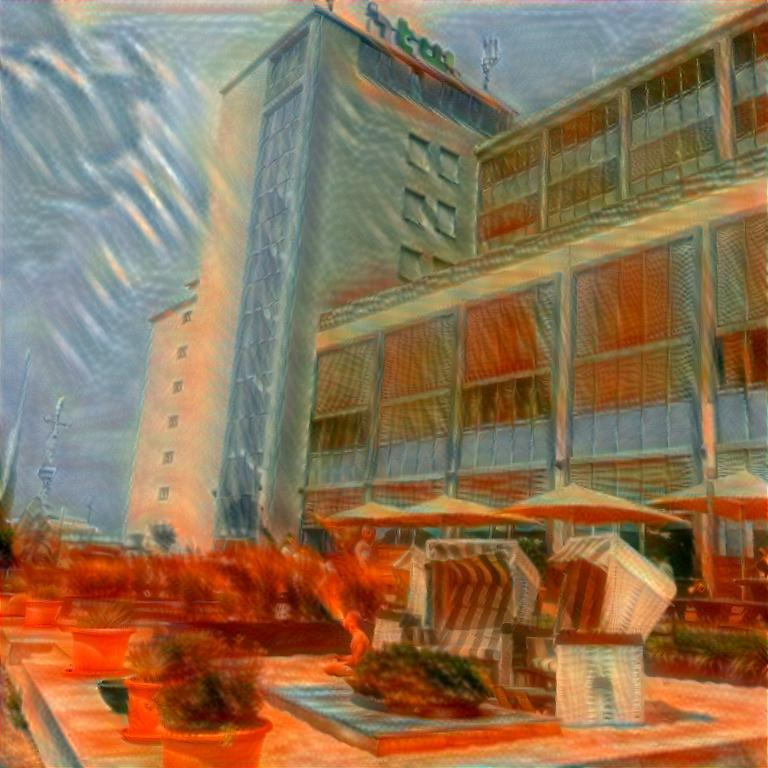
\includegraphics[width=\textwidth]{resources/content/experiments/b__the_scream__768x768__style-weight_1e+07__tv-weight_1e-06.jpg}
    \end{subfigure}
    \begin{subfigure}[h]{0.15\textwidth}
        \centering
        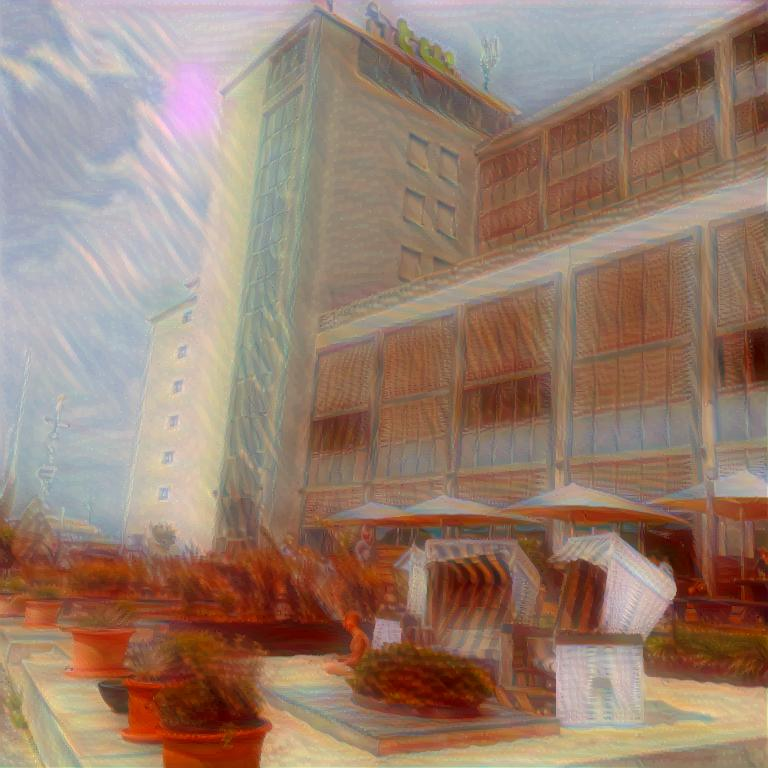
\includegraphics[width=\textwidth]{resources/content/experiments/b__the_scream__768x768__style-weight_1e+07__tv-weight_1e-05.jpg}
    \end{subfigure}
    \begin{subfigure}[h]{0.15\textwidth}
        \centering
        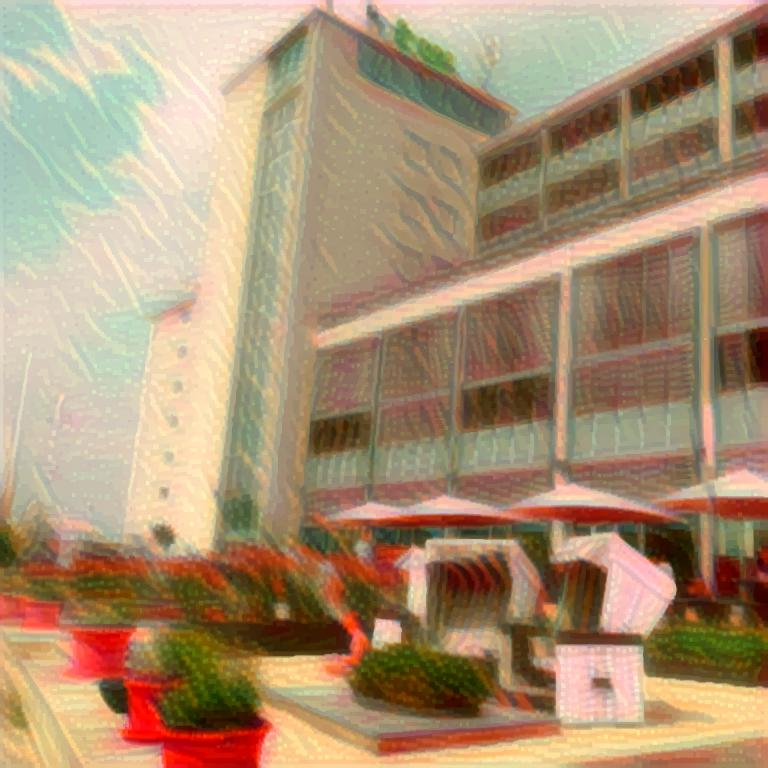
\includegraphics[width=\textwidth]{resources/content/experiments/b__the_scream__768x768__style-weight_1e+07__tv-weight_1e-04.jpg}
    \end{subfigure}
    \begin{subfigure}[h]{0.15\textwidth}
        \centering
        
\includegraphics[width=\textwidth]{resources/content/experiments/b__the_scream__768x768__style-weight_1e+07__tv-weight_1e-03.jpg}
    \end{subfigure}
    \caption{The Scream mit $ \alpha = 1 $, $ \beta = 10^{7} $, $ \gamma = 10^{-7} - 10^{-3} $}
\end{figure}

\pagebreak

\subsection{Ergebnisse}

Wie beiden Tests zu sehen ist, werden die Muster mit zunehmendem Style-Weight $ \beta $ auf dem Ausgangsbild immer stärker generierten. Mit $ b = 10^{5} $ sind bei beiden Stilen die Muster des Gemäldes kaum noch zu erkennen. Lediglich wird das Ausgangsbild den Farben des Stilbildes angepasst. Ein optisch ansprechender Effekt ergibt sich bei beiden Stilen ab $ \beta = 10^{7} $. 

Mit zunehmendem Total-Variation-Weight $ \gamma $ fließen die Farben mehr ineinander und das Ausgangsbild wird verschommener. Das ist besodners gut zu sehen bei \textit{The Starry Night} mit $ \gamma = 10^{-3} $ und \text{The Scream} mit $ \gamma = 10^{-4} $. Für \textit{The Scream} ist eine Gewichtung von $ \gamma = 10^{-3} $ bereits zu hoch gewählt. Das Ausgangsbild entwickelt sich zu einem grauen Rauschen.


\section{Auswirkungen der Netzwerkarchitekturen}

Im nächsten Experiment werden drei unterschiedlichen Bildgrößen auf unterschiedlichen Geräten auf Durchführbarkeit und Performanz getestet.
Gemessen wird die Berechnungsgeschwindigkeit beim Forward-Pass durch das Netzwerk. 

Ein bereits erster Indikator für die Performanz eines Neuronalen Netzwerks ist die Anzahl der lernbaren Parameter, die bei der Trainingsphase optimiert werden. Trainiert wurden neun unterschiedliche Netzwerke auf dem Kunstwerk \textit{The Starry Night} mit unterschiedlichen Kombinationen für $ m $ und $ s $
Dabei wurde bei allen Netzwerken eine Batch-Size von $ 16 $ und eine Learning-Rate von $ 10^{-3} $ verwendet. Die Netzwerke wurden über drei Epochen des COCO-Datensatzes trainiert. Dabei wurden die Testdaten aus dem Jahr 2014 sowie die Test-, Validierungs- und Trainingsdaten aus dem Jahr 2017 verwendet. Insgesamt handelt es sich dabei um $ 170877 $ Bilder. Insgesamt wurden die Modelle mit $ 512631 $ Bildern trainiert. Dabei dauerte die Trainingszeit auf einem Server mit einem \textit{GeForce GTX 1080 Ti}-GPU pro Modell zwischen 8 und 10 Stunden.

\begin{table}[H]
    \centering
    \begin{tabular}{ |c|c|c|c| }
        \hline
        \textbf{Name} & \textbf{Bottleneck Size $ s $} & \textbf{Multiplkator $ m $} & \textbf{Anzahl lernbarer Parameter} \\ \hline
        Netzwerk 1 & 5 & 32 & 2.006.931 \\ \hline
        Netzwerk 2 & 5 & 16 & 506.835 \\ \hline
        Netzwerk 3 & 5 & 8  & 129.267 \\ \hline

        Netzwerk 4 & 4 & 32 & 1.711.250 \\ \hline
        Netzwerk 5 & 4 & 16 & 432.722 \\ \hline
        Netzwerk 6 & 4 & 8  & 110.642 \\ \hline

        Netzwerk 7 & 3 & 32 & 1.415.569 \\ \hline
        Netzwerk 8 & 3 & 16 & 358.609 \\ \hline
        Netzwerk 9 & 3 & 8  & 92.017 \\ \hline
    \end{tabular}
    \caption{Unterschiedliche Netzwerkgrößen und ihre Parameter}
    \label{tab:networks}
\end{table}

Bei der Berechnung des Forward-Pass macht es einen Unterschied ob sie  auf dem CPU oder dem GPU eines Geräts durchgeführt wird. Neuronale Netzwerke können auf einer GPU schneller als auf einem CPU berechnet werden. Das liegt daran, dass eine GPU besonders auf die Berechnung von Matrix-Operationen (wie Sie auch bei grafischen Anwendungen verwendet werden) spezialisiert ist.

Die Daten werden beim Einsatz des GPUs in den Grafikspeicher geladen. Bei der Berechnung über den CPU wird der Arbeitsspeicher (RAM) des Geräts verwendet. Der RAM kann über die Verwendung einer Auslagerungsdatei (SWAP-Datei) virtuell erweitert werden. Somit kann verhindert werden das es zu Fehlern wegen unzureichendem Arbeitsspeicher kommt.


% Hier die Spezifikationen der Verwendenten Geräte hin.

Im folgenden werden die unterschiedlichen Netzwerkearchitekturen auf ihre Performanz getestet. Tests die wegen unzureichendem Arbeitsspeicher oder Grafikspeicher fehlschlagen werden als \textcolor{danger}{nicht durchführbar} gekennzeichnet.

\begin{table}[H]
    \centering
    \begin{tabular}{ |c|c|c|c|c| }
        \hline
        \textbf{Name} & \textbf{XPS 15 - CPU} & \textbf{XPS 15 - GPU} & \textbf{Auto - CPU} & \textbf{Auto - GPU}   \\ \hline
        Netzwerk 1 & 2.72105 & \textcolor{danger}{nicht durchführbar} & & \\ \hline
        Netzwerk 2 & 1.03105 & 0.23152                                & & \\ \hline
        Netzwerk 3 & 0.48080 & 0.13070                                & & \\ \hline
	
        Netzwerk 4 & 2.51535 & \textcolor{danger}{nicht durchführbar} & & \\ \hline
        Netzwerk 5 & 0.97727 & 0.21588                                & & \\ \hline
        Netzwerk 6 & 0.44961 & 0.12341                                & & \\ \hline

        Netzwerk 7 & 2.33272 & \textcolor{danger}{nicht durchführbar} & & \\ \hline
        Netzwerk 8 & 0.89503 & 0.20119                                & & \\ \hline
        Netzwerk 9 & 0.41804 & 0.11645                                & & \\ \hline
    \end{tabular}
    \caption{Berechnungsgeschwindigkeit für Bilder der Größe 1024 * 768 Pixel}
    \label{tab:1024x768}
\end{table}


\begin{table}[H]
    \centering
    \begin{tabular}{ |c|c|c|c|c| }
        \hline
        \textbf{Name} & \textbf{XPS 15 - CPU} & \textbf{XPS 15 - GPU} & \textbf{Auto - CPU} & \textbf{Auto - GPU}   \\ \hline
        Netzwerk 1 & 1.04234 & 0.20962 & & \\ \hline
        Netzwerk 2 & 0.41221 & 0.10425 & & \\ \hline
        Netzwerk 3 & 0.19578 & 0.05207 & & \\ \hline
	
        Netzwerk 4 & 0.95978 & 0.19487 & & \\ \hline
        Netzwerk 5 & 0.38498 & 0.09735 & & \\ \hline
        Netzwerk 6 & 0.18290 & 0.04915 & & \\ \hline

        Netzwerk 7 & 0.88858 & 0.18083 & & \\ \hline
        Netzwerk 8 & 0.35051 & 0.09149 & & \\ \hline
        Netzwerk 9 & 0.16939 & 0.04622 & & \\ \hline
    \end{tabular}
    \caption{Berechnungsgeschwindigkeit für Bilder der Größe 640 * 480 Pixel}
    \label{tab:640x480}
\end{table}


\begin{table}[H]
    \centering
    \begin{tabular}{ |c|c|c|c|c| }
        \hline
        \textbf{Name} & \textbf{XPS 15 - CPU} & \textbf{XPS 15 - GPU} & \textbf{Auto - CPU} & \textbf{Auto - GPU}   \\ \hline
        Netzwerk 1 & 0.27885 & 0.07604 & & \\ \hline
        Netzwerk 2 & 0.11639 & 0.02670 & & \\ \hline
        Netzwerk 3 & 0.05898 & 0.01308 & & \\ \hline
	
        Netzwerk 4 & 0.25559 & 0.07088 & & \\ \hline
        Netzwerk 5 & 0.10755 & 0.02511 & & \\ \hline
        Netzwerk 6 & 0.05475 & 0.01238 & & \\ \hline

        Netzwerk 7 & 0.23489 & 0.06698 & & \\ \hline
        Netzwerk 8 & 0.09734 & 0.02369 & & \\ \hline
        Netzwerk 9 & 0.05023 & 0.01172 & & \\ \hline
    \end{tabular}
    \caption{Berechnungsgeschwindigkeit für Bilder der Größe 320 * 240 Pixel}
    \label{tab:320x240}
\end{table}
